\documentclass[border=3pt,tikz]{standalone}
\usepackage{physics}
\usepackage{tikz}
\usepackage[outline]{contour} % glow around text
\usetikzlibrary{patterns,decorations.pathmorphing}
\usetikzlibrary{decorations.markings}
\usetikzlibrary{arrows.meta}
\usetikzlibrary{calc}
\tikzset{>=latex}
\contourlength{1.1pt}

\colorlet{mydarkblue}{blue!40!black}
\colorlet{myblue}{blue!30}
\colorlet{myred}{red!65!black}
\colorlet{vcol}{green!45!black}
\colorlet{watercol}{blue!80!cyan!10!white}
\colorlet{darkwatercol}{blue!80!cyan!80!black!30!white}
\tikzstyle{water}=[draw=mydarkblue,top color=watercol!90,bottom color=watercol!90!black,middle color=watercol!50,shading angle=0]
\tikzstyle{horizontal water}=[water,
top color=watercol!90!black!90,bottom color=watercol!90!black!90,middle color=watercol!80,shading angle=0]
\tikzstyle{dark water}=[draw=blue!20!black,top color=darkwatercol,bottom color=darkwatercol!80!black,middle color=darkwatercol!40,shading angle=0]
\tikzstyle{vvec}=[->,very thick,vcol,line cap=round]
\tikzstyle{force}=[->,myred,very thick,line cap=round]
\tikzstyle{width}=[{Latex[length=3,width=3]}-{Latex[length=3,width=3]}]
\begin{document}
% VENTURI EFFECT
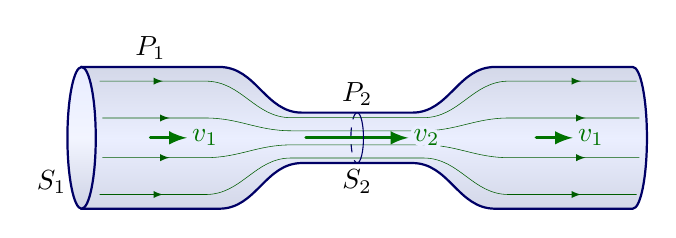
\begin{tikzpicture}
	\def\L{7.0}          % total length
	\def\m{0.20*\L}      % length pipe middle
	\def\l{0.25*\L}      % length pipe outer
	\def\rx{0.08}        % small pipe horizontal radius left
	\def\ry{0.32}        % small pipe vertical radius left
	\def\Rx{0.18}        % big pipe vertical radius right
	\def\Ry{0.90}        % big pipe vertical radius right
	\def\v{1.3}          % velocity magnitude
	\contourlength{1.5pt}
	
	% WATER
	\draw[horizontal water,thick]
	(-\L/2,\Ry) --++ (0,-2*\Ry) coordinate (A1) --++ (\l,0) to[out=0,in=180]
	(-\m/2,-\ry) --++ (\m,0) to[out=0,in=180]
	(\L/2-\l,-\Ry) --++ (\l,0) arc(-90:90:{\Rx} and \Ry) --++ (-\l,0) to[out=180,in=0]
	(\m/2,\ry) --++ (-\m,0) to[out=180,in=0] (-\L/2+\l,\Ry) -- cycle;
	\draw[water,thick]
	(-\L/2,0) ellipse({\Rx} and \Ry);
	\node[above left=2] at (A1) {$S_1$};
	\node[below=-1] at (0,-\ry) {$S_2$};
	
	% VELOCITIES
	\draw[mydarkblue,dashed]
	(0,\ry) arc(90:270:{\rx} and \ry);
	\foreach \fy in {-0.28,-0.8,0.28,0.8}{
		\coordinate (A) at ($(-\L/2,0)+({asin(\fy/1.5)}:{1.5*\Rx} and {1.5*\Ry})$);
		\coordinate (B) at ($({\L/2-\Rx},0)+({asin(\fy/1.5)}:{1.5*\Rx} and {1.5*\Ry})$);
		\draw[vcol!80!black,very thin,postaction={decorate},decoration={markings,
			mark=at position {0.13-0.02*abs(\fy)} with {\arrow{latex}},mark=at position 0.9 with {\arrow{latex}}}]
		(A) -- (-\L/2+0.9*\l,\fy*\Ry) to[out=0,in=180]
		(-0.6*\m,\fy*\ry) -- (0.6*\m,\fy*\ry) to[out=0,in=180] (\L/2-0.9*\l,\fy*\Ry) -- (B);
	}
	\draw[vvec] (-\L/2+0.5*\l,0) --++ (\v*\ry/\Ry,0) node[right=-2] {$v_1$};
	\draw[vvec] ( \L/2-0.7*\l,0) --++ (\v*\ry/\Ry,0) node[right=-2] {$v_1$};
	\draw[vvec] (-0.5*\v,0) --++ (\v,0) node[right=-2] {\contour{watercol!80}{$v_2$}};
	\draw[mydarkblue]
	(0,\ry) arc(90:-90:{\rx} and \ry);
	\node[above=-1] at (-\L/2+0.5*\l,\Ry) {$P_1$};
	\node[above=-1] at (0,\ry) {$P_2$};
	
	
\end{tikzpicture}
\end{document} 